\documentclass[12pt,letterpaper]{article}

\usepackage{amsmath, amsthm}
\usepackage{microtype, parskip}
\usepackage[comma,numbers,sort&compress]{natbib}
\usepackage{lineno}
\usepackage{docmute}
\usepackage{caption, subcaption, multirow, morefloats, rotating}
\usepackage{wrapfig}

\frenchspacing

\captionsetup[subfigure]{position = top, labelfont = bf, textfont = normalfont, singlelinecheck = off, justification = raggedright}

\begin{document}
\section{Uncertainty in environmental preference} \label{sec:uncer}
The calculation and inclusion of environmental affinity in the survival model is a statistical procedure that takes into account our uncertainty based on where fossils tend to occur. Because we cannot directly observe if a fossil taxon had occurrences restricted to only a single environment, instead we can only estimate its affinity with uncertainty. One advantage of using a Bayesian analytical approach is that both parameters and data are considered random samples from some underlying distribution, which means that is is possible to model the uncertainty in our covariates of interest \citep{Gelman2013d}. My approach is conceptually similar to \citet{Simpson2009} but instead of obtaining a single point estimate, an entire posterior distribution is estimated.

The first step is to determine the probability \(\theta\) at which genus \(i\) occurs in an epicontinental settings based on its own pattern of occurrences. Define \(e_{i}\) as the number of occurrences of genus \(i\) in an epicontiental sea and \(o_{i}\) as the number of occurrences of genus \(i\) not in an epicontinental sea (e.g. open ocean). Because the value of interest is the probability of occurring in an epicontinental environment, given the observed fossil record, I assume that probability follows a binomial distribution. We can then define our sampling statement as
\begin{equation}
  e_{i} \sim \mathrm{Binomial}(e_{i} + o_{i}, \theta_{i}).
  \label{eq:epi_lik}
\end{equation}
I used a flat prior for \(\theta_{i}\) defined as \(\theta_{i} \sim \mathrm{Beta}(1, 1)\). Because the beta distribution is the conjugate prior for the binomial distribution, the posterior is easy to compute in closed form. The posterior probability of \(\theta\) is then 
\begin{equation}
  \theta_{i} \sim \mathrm{Beta}(e_{i} + 1, o_{i} + 1)
  \label{eq:epi_post}
\end{equation}

It is extremely important, however, to take into account the overall environmental occurrence probability of all other genera present at the same time as genus \(i\). This is incorporated as an additional probability \(\Theta\). Define \(E_{i}\) as the total number of other fossil occurrences (exceptfor genus \(i\)) in epicontinental seas during stages where \(i\) occurs and \(O_{i}\) as the number of other fossil occurrences not on epicontinental seas. We can then define the sampling statement as
\begin{equation}
  E_{i} \sim \mathrm{Binomial}(E_{i} + O_{i}, \Theta_{i}).
  \label{eq:bck_lik}
\end{equation}
Again, I used a flat prior of \(\Theta_{i}\) defined as \(\Theta_{i} \sim \mathrm{Beta}(1, 1)\). The posterior of \(\Theta\) is then simply defined as

\begin{equation}
  \Theta_{i} \sim \mathrm{Beta}(E_{i} + 1, O_{i} + 1)
  \label{eq:bck_post}
\end{equation}

I then define the environmental affinity of genus \(i\) as \(v_{i} = \theta_{i} - \Theta_{i}\). \(v_{i}\) is a value that can range between -1 and 1, where negative values indicate that genus \(i\) tends to occur more frequently in open ocean environments than background while positive values indicate that genus \(i\) tends to occur in epicontiental environments.

While this approach is noticeably more complicated than previous ones \citep{Foote2006,Miller2001,Simpson2009,Kiessling2007a} there are some important benefits to both using a continuous measure of affinity as well directly modeling our uncertainty. In order to show some of these benefits, I performed a simulation analysis of how modal/maximum \textit{a posteriori} (MAP) estimates versus full posterior estimates.

In this simulation, I first defined the ``background'' epicontinental occurrence \(\theta_{b}\) as 0.50 with a small amount of noise. This was represented as a beta distribution 

\begin{equation}
  \Theta_{b} = \mathrm{Beta}(\alpha = 2500, \beta = 2500). 
  \label{eq:bck_sim}
\end{equation}
This choice of parameters for the distribution reflects the average number of background occurrences for either epicontinental or open ocean environments per genus.

Using this background occurrence ratio, I randomly generated the occurrence patterns of 1000 simulated taxa. This was done at multiple sample sizes (1, 2, 3, 4, 5, 10, 25, 50, 100) in order to demonstrate the effects of increasing sample size on the confidence of environmental affinity. For each simulated taxon I calculated the full posterior distribution while assuming a flat Beta prior (\(\mathrm{Beta}(1, 1)\)). Using the full posterior I calculated the MAP probability of occurring in epicontinental environments. The environmental affinity was calculated for each of the simulated taxa using both the full posterior and the MAP estimate. In this toy example, environmental affinity can range between -0.5 and 0.5.

As should be expected, as sample size increases the distribution of MAP estimates converge on the true value (Fig. \ref{fig:env_mode}). For taxa with less than 10 occurrences, the MAP estimate is biased towards extreme values. Note that the mode of the beta distribution is not defined for situations where there were 0 draws of one of the environmental conditions. Instead, the vertical line is based entirely on the observed occurrences which are technically the modal estimates because they are the most frequently occurring/highest density.

In contrast, we can compare the true occurrence probability distribution versus the posterior estimate for a given sample (Fig. \ref{fig:env_post}). When sample sizes are low, posterior estimates are flat and represent a compromise between the likelihood and the flat prior (Eq. \ref{eq:epi_post}). Because of this, estimates from small sizes are less likely to be overly biased towards the extremes. This is further emphasized by inspection of the estimates of environmental affinity for the simulated taxa (Fig. \ref{fig:env_diff}). Posterior estimates from simulated taxa with small sample size have a much broader distribution that both allows for the extreme observation but still captures the ``true'' value (0). 


By defining environmental preference as the difference in full posterior estimates of occurrence probability, it is possible to include taxa with low sample sizes that are normal discarded \citep{Foote2006,Miller2001,Simpson2009,Kiessling2007a}. Additionally, 55+\% of observed Paleozoic brachiopod genera have less than 10 occurrences which is the range of sample sizes where MAP (or ML) estimates would be potentially most biased. This is preferable to finding the difference between the MAP estimates (blue line; Fig. \ref{fig:env_diff}).

% behavior of MAP estimates
%   as sample size increases, converge on true (10+)
% behavior of posterior
%   compromise between likelihood of data occurrences and (flat) prior
%   really important for small sample sizes
%   at 10+ makes no difference anymore
%   this is also kind obvious from the estimates of \(v\)
% how many taxa have less than 10 occurrences? \approx 55\%

\begin{figure}[ht]
  \centering
  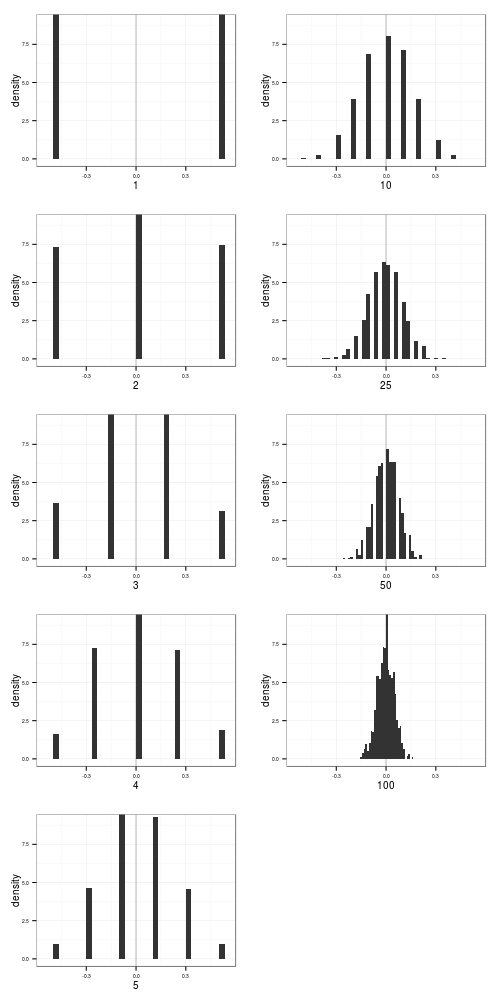
\includegraphics[height = \textheight,width=\textwidth,keepaspectratio=true]{figure/env_mode_dist}
  \caption{Histograms of the distributions of from the beta distribution defined in Eq. \ref{eq:bck_sim}. As to be expected, as sample size increases the draws better resemble the underlying true distribution. Sample size is indicated as the label of the x-axis, increasing in column major order.}
  \label{fig:env_mode}
\end{figure}

\begin{figure}[ht]
  \centering
  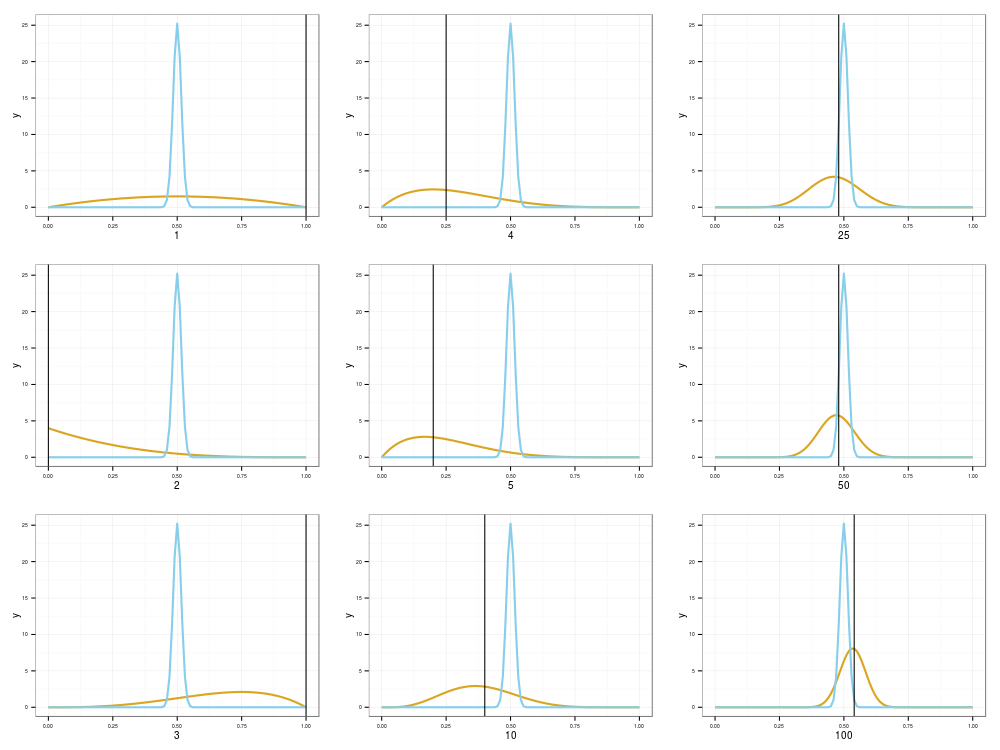
\includegraphics[height = \textheight,width=\textwidth,keepaspectratio=true]{figure/env_post_inspect}
  \caption{Comparisons of the underlying distribution (blue) to posterior estimates based on increasing sample size (gold). Each posterior estimate is represented for only a single realization of draws, each with sample size indicated as the x-axis label (increasing in column major order). Black vertical lines correspond to the MAP estimate of the simulated taxon's affinity. This stands in contrast to the posterior distribution of expected affinity in gold.}
  \label{fig:env_post}
\end{figure}

\begin{figure}[ht]
  \centering
  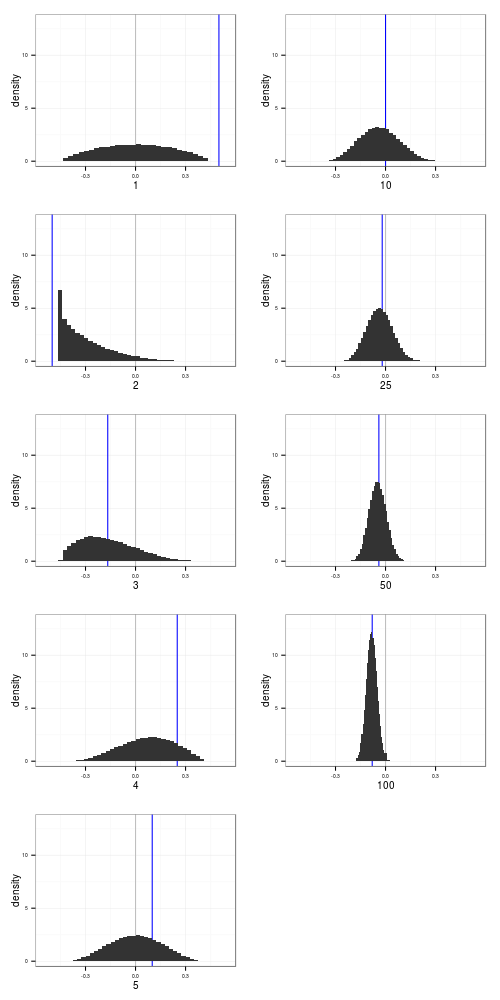
\includegraphics[height = \textheight,width=\textwidth,keepaspectratio=true]{figure/env_diff}
  \caption{Histograms of the difference in the underlying occurrence distribution and the posterior distribution estimates from the previous graph (Fig. \ref{fig:env_post}). The ``true'' value is included in all distributions of environmental affinities. Each affinity estimate is represented for only a single realization of draws, each with sample size indicated as the x-axis label (increasing in column major order). Blue vertical lines correspond to the difference in MAP estimates between the underlying distribution and the simulated taxon's draws. This stands in contrast to the distribution of the differences between the simulated taxon and background.}
  \label{fig:env_diff}
\end{figure}

\section{Survival model} \label{sec:survival}

The simplest model of genus duration includes no covariate or structural information. Define \(y_{i}\) as the duration in stages of genus \(i\), where \(i = 1, \dots, n\) and \(n\) is the number of observed genera. These two models are them simply defined as
\begin{equation}
  \begin{aligned}
    y_{i} &\sim \mathrm{Exponential}(\lambda) \\
    y_{i} &\sim \mathrm{Weibull}(\alpha, \sigma).
  \end{aligned}
  \label{eq:simple}
\end{equation}
\(\lambda, \alpha, \text{and} \sigma\) are all defined for all positive reals. Note that \(\lambda\) is a ``rate'' or inverse-scale while \(\sigma\) is a scale parameter, meaning that \(\frac{1}{\lambda} = \sigma\).

These simple models can then be expanded to include covariate information as predictors by reparameterizing \(\lambda\) or \(\sigma\) as a regression \citep{Klein2003}. Each of the covariates of interest is given its own regression coefficient (e.g. \(\beta_{r}\)) along with an intercept term \(\beta_{0}\). There are some additional complications to the parameterization of \(\sigma\) associated with the inclusion of \(\alpha\) as well as for interpretability \citep{Klein2003}. Both of these are then written as
\begin{equation}
  \begin{aligned}
    \lambda_{i} &= \exp(\beta_{0} + \beta_{r} r_{i} + \beta_{v} v_{i} + \beta_{v^{2}} v_{i}^{2} + \beta_{m} m_{i}) \\
    \sigma_{i} &= \exp\left(\frac{-(\beta_{0} + \beta_{r} r_{i} + \beta_{v} v_{i} + \beta_{v^{2}} v_{i}^{2} + \beta_{m} m_{i})}{\alpha}\right).
  \end{aligned}
  \label{eq:regression}
\end{equation}
The quadratic term for environmental affinity \(v\) is to allow for the possible nonlinear relationship between environmental affinity and extinction risk.

The models which incorporate both equations \ref{eq:simple} and \ref{eq:regression} can then be further expanded to allow all of the \(\beta\) coefficients, including \(\beta_{0}\), to vary with origination cohort while also modeling their covariance and correlation. This is called a varying-intercepts, varying-slopes model \citep{Gelman2007}. It is much easier to represent and explain how this is parameterized using matrix notation. First, define \(\mathbf{B}\) as \(k \times J\) matrix of the \(k\) coefficients including the intercept term (\(k = 5\)) for each of the \(J\) cohorts. Second, define \(\mathbf{X}\) as a \(n \times k\) matrix where each column is one of the covariates of interest. Importantly, \(\mathbf{X}\) includes a columns of all 1s which correspond to the constant term \(\beta_{0}\). Third, define \(j[i]\) as the origination cohort of genus \(i\), where \(j = 1, \dots, J\) and \(J\) is the total number of observed cohorts. We then rewrite \(\lambda\) and \(\sigma\) of equation \ref{eq:regression} in matrix notation as
\begin{equation}
  \begin{aligned}
    \lambda_{i} &= \exp(\mathbf{X}_{i} B_{j[i]}) \\
    \sigma_{i} &= \exp\left(\frac{-(\mathbf{X}_{i} B_{j[i]})}{\alpha}\right). 
  \end{aligned}
  \label{eq:multivariate}
\end{equation}

Because \(B\) is a matrix, I use a multivariate normal prior with unknown vector of means \(\mu\) and covariance matrix \(\Sigma\). This is written as 
\begin{equation}
  B \sim \mathrm{MVN}(\vec{\mu}, \Sigma)
  \label{eq:beta_prior}
\end{equation}
where \(\vec{\mu}\) is length \(k\) vector representing the overall mean of the distributions of \(\beta\) coefficients. \(\Sigma\) is a \(k \times k\) covariance matrix of the \(\beta\) coefficients.

What remains is assigning priors the elements of \(\vec{\mu}\) and the covariance matrix \(\Sigma\). All elements of \(\vec{\mu}\) except for \(\mu_{r}\) were given horseshoe priors \citep{Carvalho2010,Carvalho2009} while \(\mu_{r}\) was given an informative normal prior (\(\mu_{r} \sim \mathcal{N}(-1, 1)\). Horseshoe priors are a strong regularizing priors with effectively infinite density at 0 and heavy, Cauchy-like tails \citep{Carvalho2010,Carvalho2009} which allow weakly inferred effects to be strongly drawn towards 0 while truly strong effects can remain large. The horseshoe prior consists of a normal distribution with scale term that is the product between a global shrinkage parameter \(\nu\) and a locak shrinkage parameter \(\psi\) unique to each of the parameters of interest. These parameters are themselves given half-Cauchy priors (Eq. \ref{eq:exp_total} and \ref{eq:wei_total}).

The prior for \(\Sigma\) is a bit more complicated due to its multivariate nature. Following the \citet{stan-manual:2014}, I modeled the scale terms separate from the correlation structure of the coefficients. This is possible because of the relationship between a covariance and a correlation matrix, defined as 
\begin{equation}
  \Sigma_{B} = \text{Diag}(\vec{\tau}) \Omega \text{Diag}(\vec{\tau})
  \label{eq:covcor}
\end{equation}
where \(\vec{\tau}\) is a length \(k\) vector of variances and Diag(\(\tau\)) is a diagonal matrix.

I used a LKJ prior distribution for correlation matrix \(\Omega\) as recommended by \citet{stan-manual:2014}. The LKJ distribution is a single parameter multivariate distribution where values of the parameter \(\eta\) greater than 1 concentrate density at the unit correlation matrix, which corresponds to no correlation between the \(\beta\) coefficients. The scale parameters, \(\vec{\tau}\), are given weakly informative half-Cauchy (C\(^{+}\)) priors following \citet{Gelman2006a}.



\section{Censored observations} \label{sec:cen}
A key aspect of survival analysis is the inclusion of censored, or incompletely observed, data points \citep{Ibrahim2001,Klein2003}. The two classes of censored observations encountered in this study were right and left censored observations. Right censored genera are those that did not go extinct during the window of observation, or genera that are still extant. Left censored observations are those taxa for which we know only an upper limit on their duration.

In the context of this study, I considered all genera that had a duration of only one geologic stage to be left censored as we do not have a finer degree of resolution. 

The key function for modeling censored observations is the survival function, or \(S(t)\). \(S(t)\) corresponds to the probability that a genus having existed for \(t\) stages will not have gone extinct while \(h(t)\) corresponds to the instantaneous extinction rate at taxon age \(t\) \cite{Klein2003}. For an exponential model, \(S(t)\) is defined as
\begin{equation}
  S(t) = \exp(-\lambda t),
  \label{eq:exp_surv}
\end{equation}
and for the Weibull distribution \(S(t)\) is defined as
\begin{equation}
  S(t) = \exp\left(-\left(\frac{t}{\sigma}\right)^{\alpha}\right).
  \label{eq:wei_surv}
\end{equation}
\(S(t)\) is equivalent to the complementary cumulative distribution function, \(1 - F(t)\) \citep{Klein2003}. 

For right censored observations, instead of calculating the likelihood as normal (Eq. \ref{eq:multivariate}) the likelihood of an observation is evaluated using \(S(t)\). Conceptually, this approach calculates the likelihood of observing a taxon that existed for at least that long. For left censored data, instead the likelihood is calculated using \(1 - S(t)\) which corresponds to the likelihood of observing a taxon that existed no longer than \(t\).

The full likelihood statements incorporating fully observed, right censored, and left censored observations are then
\begin{equation}
  \begin{aligned}
    \mathcal{L} &\propto \prod_{i \in C} \mathrm{Exponential}(y_{i} | \lambda) \prod_{j \in R} S(y_{j} | \lambda) \prod_{k \in L} \left(1 - S(y_{k} | \lambda)\right) \\
    \mathcal{L} &\propto \prod_{i \in C} \mathrm{Weibull}(y_{i} | \alpha, \sigma) \prod_{j \in R} S(y_{j} | \alpha, \sigma) \prod_{k \in L} \left(1 - S(y_{k} | \alpha, \sigma)\right)
  \end{aligned}
  \label{eq:censored_likelihood}
\end{equation}
where \(C\) is the set of all fully observed taxa, \(R\) the set of all right censored taxa, and \(L\) the set of all left-censored taxa.


\section{Widely applicable information criterion} \label{sec:waic}
WAIC can be considered a fully Bayesian alternative to the Akaike information criterion, where WAIC acts as an approximation of leave-one-out cross-validation which acts as a measure of out-of-sample predictive accuracy \citep{Gelman2013d}. WAIC is calculated starting with the log pointwise posterior predictive density calculated as
\begin{equation}
  \mathrm{lppd} = \sum_{i = 1}^{n} \log \left(\frac{1}{S} \sum_{s = 1}^{S} p(y_{i}|\Theta^{S})\right),
  \label{eq:lppd}
\end{equation}
where \(n\) is sample size, \(S\) is the number posterior simulation draws, and \(\Theta\) represents all of the estimated parameters of the model. This is similar to calculating the likelihood of each observation given the entire posterior. A correction for the effective number of parameters is then added to lppd to adjust for overfitting. The effective number of parameters is calculated, following the recommendations of \citet{Gelman2013d}, as
\begin{equation}
  p_{\mathrm{WAIC}} = \sum_{i = 1}^{n} V_{s = 1}^{S} (\log p(y_{i}|\Theta^{S})).
  \label{eq:pwaic}
\end{equation}
where \(V\) is the sample posterior variance of the log predictive density for each data point.

Given both equations \ref{eq:lppd} and \ref{eq:pwaic}, WAIC is then calculated
\begin{equation}
  \mathrm{WAIC} = \mathrm{lppd} - p_{\mathrm{WAIC}}.
  \label{eq:waic}
\end{equation}
When comparing two or more models, lower WAIC values indicate better out-of-sample predictive accuracy. Importantly, WAIC is just one way of comparing models. When combined with posterior predictive checks it is possible to get a more complete understanding of a model's fit to the data.

\end{document}
